% !TEX TS-program = pdflatex
% !TEX encoding = UTF-8 Unicode

% Matthew Urffer Master Thesis
% 
% Methods
%
\section{Spectra Methods}

%%%%%%%%%%%%%%%%%%%%%%%%%%%%%%%%%%%%%%%%%%%%%%%%%%%%%%%%%%%%%%%%%%%%%%%%%%%%%%%
%                                                                             %
%                                   FACILITIES                                %
%                                                                             %
%%%%%%%%%%%%%%%%%%%%%%%%%%%%%%%%%%%%%%%%%%%%%%%%%%%%%%%%%%%%%%%%%%%%%%%%%%%%%%%

\subsection{Facilities}
%%%%%%%%%%%%%%%%%%%%%%%%%%%%%%%%%%%%%%%%%%%%%%%%%%%%%%%%%%%%%%%%%%%%%%%%%%%%%%%
\begin{frame}{Button Sources}
	\centering
	Alpha Sources
	\begin{table}[h]
		\tiny
		\begin{tabular}{c | c c}
		Source & Half-Life & Energy (MeV) \\
		\hline
		\hline
		${}^{232}$Th & $1.4\times10^{10}$ yr & 4.012 \\
		${}^{240}$Pu & $6.5\times10^{3}$ yr & 5.17 (76\%) 5.12 (24\%) \\
		${}^{241}$Am & 433 yr & 5.48 (85\%) 5.44 (12\%) \\
		${}^{239}$Pu, ${}^{241}$Am, ${}^{244}$Cm  & various & various \\
		\end{tabular}
	\end{table}
	Beta Sources
	\begin{table}[h]
		\tiny
		\begin{tabular}{c | c c}
		Source & Half-Life & Endpoint Energy (MeV)\\
		\hline
		\hline
		${}^{14}$C &  5,730 yr & 0.156 \\
		${}^{36}$Cl & $3.08\times10^{5}$ yr & 0.714 \\
		${}^{36}$Ni &  92 yr & 0.067 \\
		${}^{99}$Tc & $2.12\times10^{5}$ yr & 0.292 \\
		\end{tabular}
	\end{table}
\end{frame}

%%%%%%%%%%%%%%%%%%%%%%%%%%%%%%%%%%%%%%%%%%%%%%%%%%%%%%%%%%%%%%%%%%%%%%%%%%%%%%%
\begin{frame}{Gamma Irridiator}
\begin{columns}[onlytextwidth]
\begin{column}{0.45\textwidth}
	\begin{itemize}
		\item Desire a 10 mR/hr Gamma Field
		\item Solution is a 100 $\mu$Ci ${}^{60}$Co source
		\item Shielded by lead
	\end{itemize}
\end{column}
\begin{column}{0.45\textwidth}
	\centering
	\begin{figure}
		\includegraphics[width=0.8\textwidth]{GammaIrridiator.eps}
		\label{fig:GammaIrridiator}
		\caption{Gamma Irridiator}
	\end{figure}
\end{column}
\end{columns}
\end{frame}

%%%%%%%%%%%%%%%%%%%%%%%%%%%%%%%%%%%%%%%%%%%%%%%%%%%%%%%%%%%%%%%%%%%%%%%%%%%%%%%
\begin{frame}{Neutron Irridiator}
\begin{columns}[onlytextwidth]
\begin{column}{0.45\textwidth}
	\small
	\begin{itemize}
		\item Source is 0.59 $\mu$g ${}^{252}$Cf
		\item Encased in HDPE Box
		\item Two detector wells
		\begin{itemize}
			\tiny
			\item Lead Well
			\item Cadmium Well
		\end{itemize}
	\end{itemize}
\end{column}
\begin{column}{0.45\textwidth}
	\begin{figure}
		\centering
		\includegraphics[height=0.25\textheight]{NeutronIrridiator_CAD.eps}
		\caption{CAD Rendering of Neutron Irridiator}
		\label{fig:NeutronIrridiatorCAD}
		\includegraphics[height=0.25\textheight]{NeutronIrridiator_MCNP.eps}
		\caption{MCNPX Rendering of Neutron Irridiator}
		\label{fig:NeutronIrridiatorMNCPX}
	\end{figure}
\end{column}
\end{columns}
\end{frame}

%%%%%%%%%%%%%%%%%%%%%%%%%%%%%%%%%%%%%%%%%%%%%%%%%%%%%%%%%%%%%%%%%%%%%%%%%%%%%%%
\begin{frame}{Neutron Irridiator (Spectra)}
\begin{columns}[onlytextwidth]
\begin{column}{0.45\textwidth}
	\begin{itemize}
		\small
		\item Lead Well
		\begin{itemize}
			\tiny
			\item Neutrons of all energies
			\item Lead to match photon attenuation of cadmium
		\end{itemize}
		\small
		\item Cadmium Well
		\begin{itemize}
			\tiny
			\item Cadmium cutoff is about 0.5 eV
			\item Well response is to fast neutrons
			\item Shielding of photons from cadmium
		\end{itemize}
		\small 
		\item Subtraction is preformed between the two response to extract the response from thermal neutrons
	\end{itemize}
\end{column}
\begin{column}{0.45\textwidth}
	\begin{figure}
		\centering
		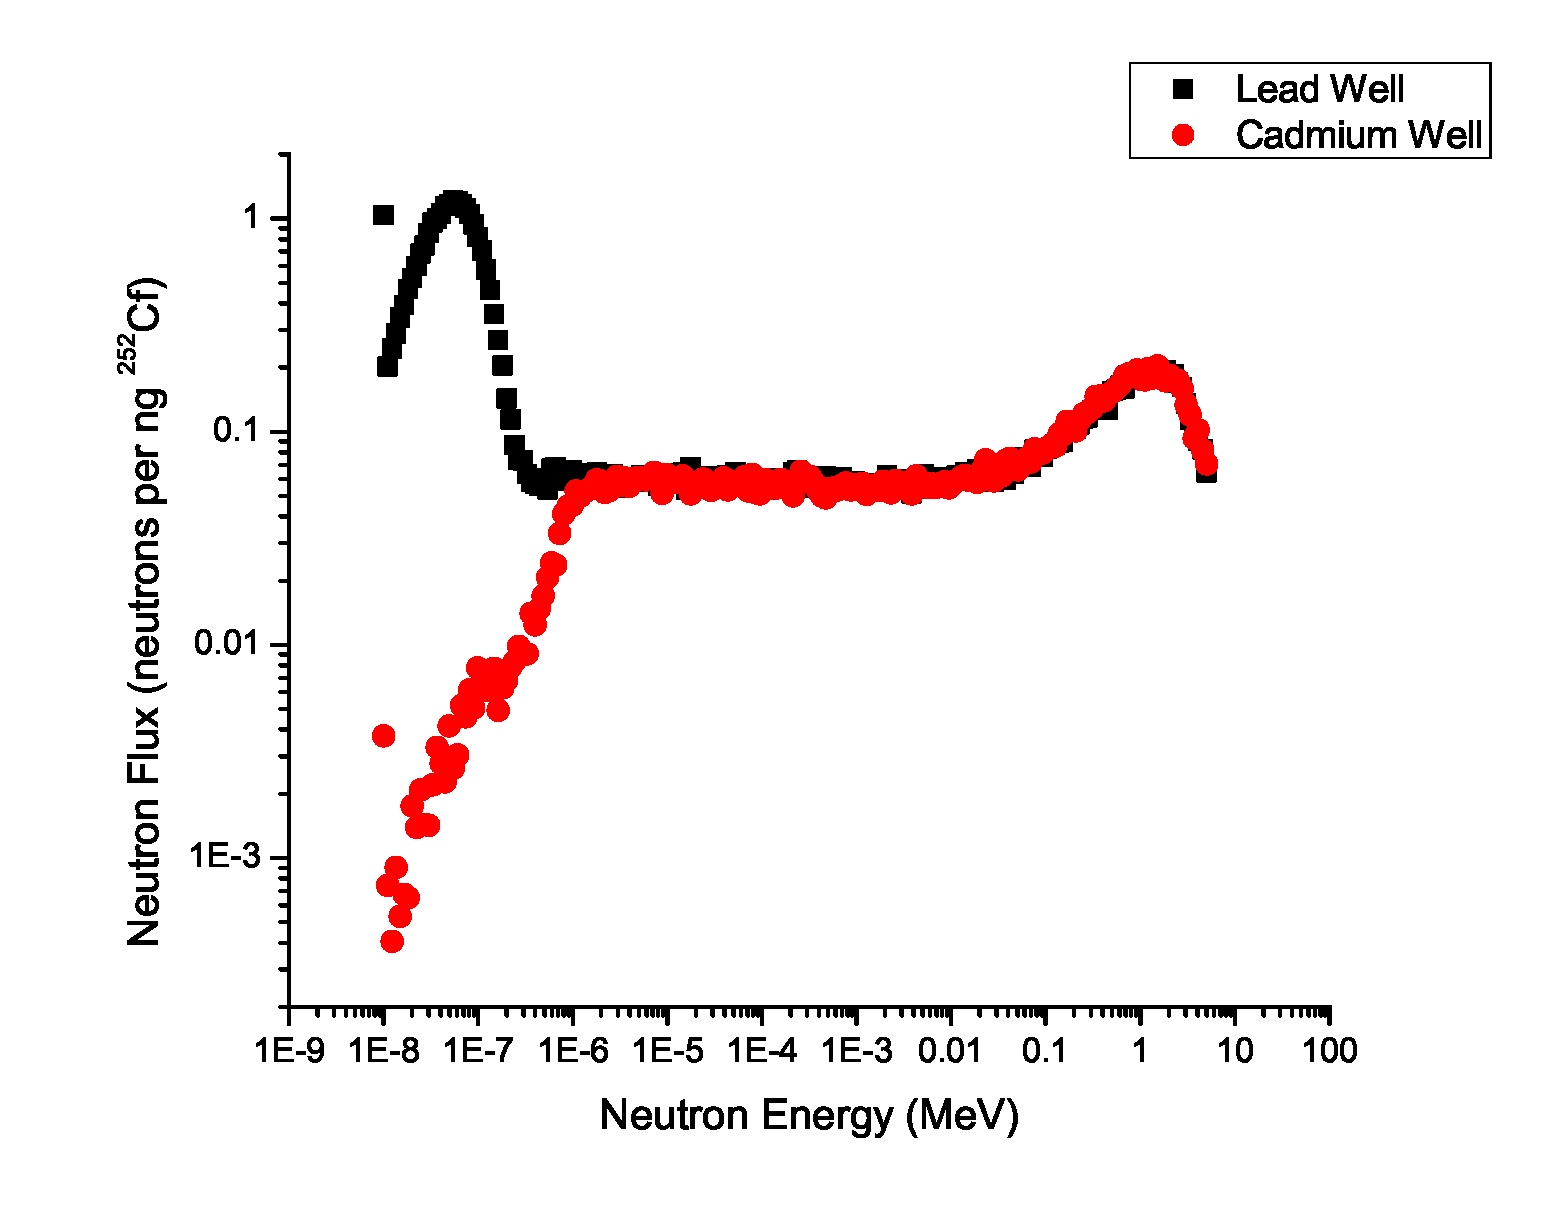
\includegraphics[width=\textwidth]{Graph19N.eps}
		\caption{Simulated Lead and Cadmium Well Spectra}
		\label{fig:SimPbCdSpectra}
	\end{figure}
\end{column}
\end{columns}
\end{frame}
%%%%%%%%%%%%%%%%%%%%%%%%%%%%%%%%%%%%%%%%%%%%%%%%%%%%%%%%%%%%%%%%%%%%%%%%%%%%%%%
\begin{frame}{Spectra Electronics}
\begin{columns}[onlytextwidth]
\begin{column}{0.45\textwidth}
	\small 
	Measurement Protocol
	\begin{itemize}
		\tiny
		\item Verify instrument gains are stable
		\begin{itemize}
			\tiny
			\item GS20 (${}^6$Li glass) is used as the standard
			\item Set voltage and coarse gain, adjust fine gain
		\end{itemize}
		\tiny
		\item Obtain a spectra from an alpha (${}^{241}$Am) 
		\item Obtain a spectra from a beta (${}^{36}$Cl)
		\item Obtain a lead well neutron spectra
		\item Obtain a cadmium well neutron spectra
		\item Obtain a gamma irridiator spectra
	\end{itemize}
\end{column}
\begin{column}{0.45\textwidth}
	\begin{figure}
		\centering
		\includegraphics[height=0.5\textwidth]{ElectronicsSpectra.eps}
		\caption{Electronic Setup for Spectra}
		\label{fig:ElectronicsSpectra}
	\end{figure}
\end{column}
\end{columns}
\end{frame}
%%%%%%%%%%%%%%%%%%%%%%%%%%%%%%%%%%%%%%%%%%%%%%%%%%%%%%%%%%%%%%%%%%%%%%%%%%%%%%%
%                                                                             %
%                             ANALYSIS METHDOS                                %
%                                                                             %
%%%%%%%%%%%%%%%%%%%%%%%%%%%%%%%%%%%%%%%%%%%%%%%%%%%%%%%%%%%%%%%%%%%%%%%%%%%%%%%
\subsection{Analysis Methods}
%%%%%%%%%%%%%%%%%%%%%%%%%%%%%%%%%%%%%%%%%%%%%%%%%%%%%%%%%%%%%%%%%%%%%%%%%%%%%%%
\begin{frame}{Spectra Average}
	\begin{itemize}
		\item Thin films do not have clearly define features
		\item Spectra averages defined to create a feature
	\end{itemize}
\begin{columns}[onlytextwidth]
\begin{column}{0.45\textwidth}
	\newtheorem{thm4}{Spectra Average}
	\begin{thm4}<1->
		$$<\mu> = \frac{\int_{0}^{\infty}x\cdot f(x)dx}{\int_{0}^{\infty}f(x)dx} $$
		where:
		\begin{itemize}
			\tiny
			\item $<\mu>$ is the average of the spectra
			\item $f(x)$ is the spectra
			\item $x$ is a channel number
		\end{itemize}
	\end{thm4}
\end{column}
\begin{column}{0.45\textwidth}
	\begin{figure}
		\centering
		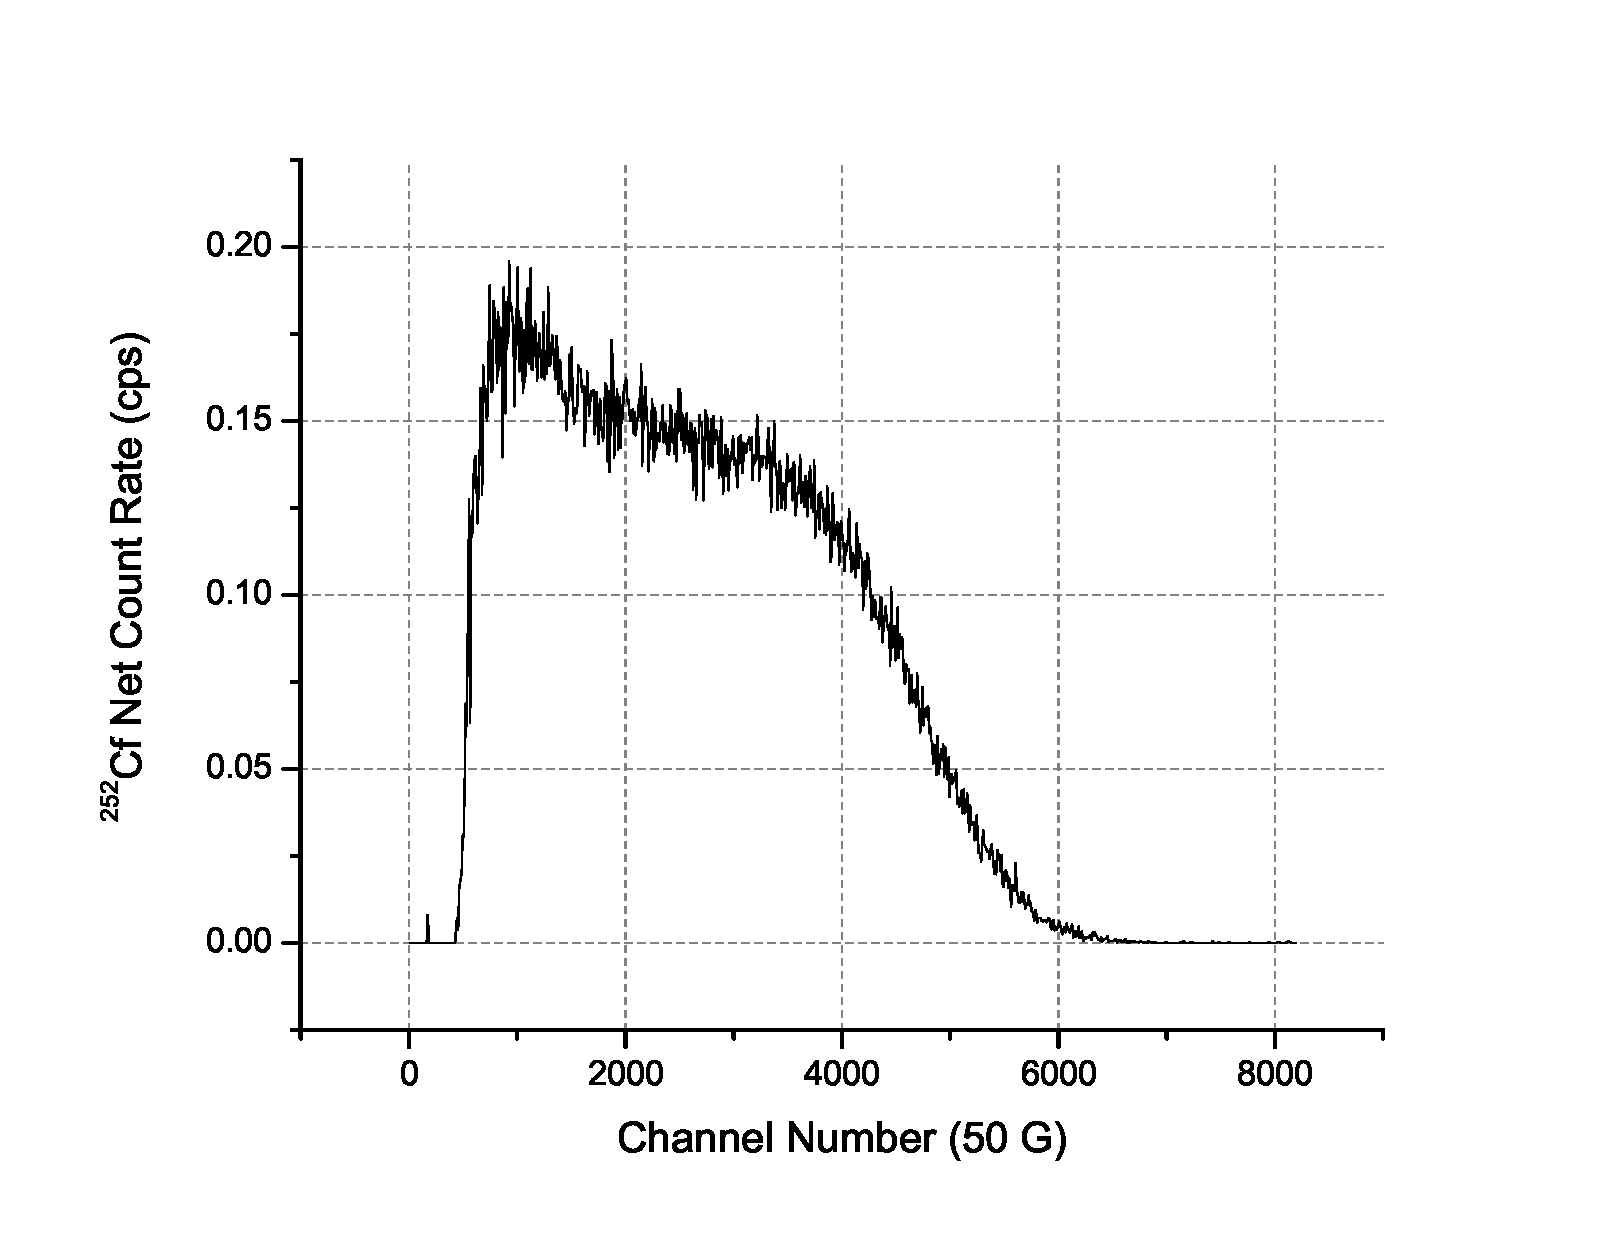
\includegraphics[width=\textwidth]{StrechedPEN-Neutron.eps}
		\caption{Example Neutron Spectra}
	\end{figure}
\end{column}
\end{columns}
\end{frame}
%%%%%%%%%%%%%%%%%%%%%%%%%%%%%%%%%%%%%%%%%%%%%%%%%%%%%%%%%%%%%%%%%%%%%%%%%%%%%%%
\begin{frame}{Pulse Height Defect}
	\newtheorem{thm5}{Pulse Height Defect}
	\begin{thm5}<1->
	\tiny
	$$ PHD_{GS20} = \frac{\dfrac{n_{peak}}{4.78\;\text{MeV}}}{\dfrac{CE_\gamma}{1.038\;\text{MeV}}} $$
		where:
		\begin{itemize}
			\tiny
			\item $PHD_{GS20}$ is the pulse height defect for GS20
			\item $n_{peak}$ is the location of the peak in the neutron spectra
			\item $CE_\gamma$ is the Compton Edge of the Gamma Spectra
		\end{itemize}
	\end{thm5}
	\newtheorem{thm6}{Pulse Height Defect (Sample)}
	\begin{thm6}<1->
	\tiny
	$$ PHD_{Sample} = PHD_{GS20} \frac{<n>_{sample}}{<n>_{GS20}} $$
		where:
		\begin{itemize}
			\tiny
			\item $PHD_{GS20}$ is the pulse height defect for GS20
			\item $<n>_{sample}$ is the average of the sample's neutron spectra
			\item $<n>_{GS20}$ is the average of GS20's neutron spectra
		\end{itemize}
	\end{thm6}
\end{frame}
%%%%%%%%%%%%%%%%%%%%%%%%%%%%%%%%%%%%%%%%%%%%%%%%%%%%%%%%%%%%%%%%%%%%%%%%%%%%%%%
\begin{frame}{Light Yield}
	\newtheorem{thm7}{Light Yield}
	\begin{thm7}<1->
	\tiny
	$$ LY_{n} = 3,800 \frac{\text{Photons}}{\text{MeV}}\frac{<n>_{sample}}{<n>_{GS20}} $$
	$$ LY_{\beta} = 3,800 \frac{\text{Photons}}{\text{MeV}}\frac{<\beta>_{sample}}{<\beta>_{GS20}} $$
	$$ LY_{\gamma} = 3,800 \frac{\text{Photons}}{\text{MeV}}\frac{<\gamma>_{sample}}{<\gamma>_{GS20}} $$
		where:
		\begin{itemize}
			\tiny
			\item $<n>_{sample}$ is the average of the sample's neutron spectra
			\item $<n>_{GS20}$ is the average of GS20's neutron spectra
			\item $<\beta>_{sample}$ is the average of the sample's beta (${}^{36}$Cl) spectra
			\item $<\beta>_{GS20}$ is the average of GS20's bet (${}^{36}$Cl) spectra
			\item $<\gamma>_{sample}$ is the average of the sample's gamma (${}^{60}$Co) spectra
			\item $<\gamma>_{GS20}$ is the average of GS20's gamma (${}^{60}$Co) spectra
		\end{itemize}
	\end{thm7}
\end{frame}
%%%%%%%%%%%%%%%%%%%%%%%%%%%%%%%%%%%%%%%%%%%%%%%%%%%%%%%%%%%%%%%%%%%%%%%%%%%%%%%
\begin{frame}
	\newtheorem{thm8}{Gamma Intrinsic Efficiency}
	\begin{thm8}<1->
		$$ \epsilon_{int,\gamma} = \frac{\int_{MLLD}^{\infty}{f(x)dx}}{\text{Particles Incident}} $$
	where:
	\begin{itemize}
		\tiny
		\item $MLLD$ is the mathematical lower level discriminator
		\item $f(x)$ is the spectra
		\item $\text{Particles Incident}$ is the number of incident particles
	\end{itemize}
	\end{thm8}
	\newtheorem{rmk1}{Mathematical Lower Level Discriminator}
	\begin{rmk1}
		\tiny
		Mathematical lower level discriminator (MLLD) is defined to be the channel at which $\epsilon_{int,\gamma} \leq 10^{-6}$
	\end{rmk1}

	\begin{itemize}
		\tiny
		\item MLLD for a film is determined from a ${}^{60}$Co measurement
		\item Source produces a 10 mR/hr field at detector surface
		\item Particles incident determined from simulation
	\end{itemize}
\end{frame}
%%%%%%%%%%%%%%%%%%%%%%%%%%%%%%%%%%%%%%%%%%%%%%%%%%%%%%%%%%%%%%%%%%%%%%%%%%%%%%%
\begin{frame}[allowframebreaks]
    \frametitle{Gamma Intrinsic Efficiency Example}
	\begin{figure}
		\centering
		\includegraphics[height=0.5\textheight]{CartoonIntEffSimple.eps}
		\caption{Determination of the MLLD for a PEN film}
		\label{fig:CartoonIntEffSimple}
	\end{figure}
%\end{frame}
%%%%%%%%%%%%%%%%%%%%%%%%%%%%%%%%%%%%%%%%%%%%%%%%%%%%%%%%%%%%%%%%%%%%%%%%%%%%%%%
%\begin{frame}{Gamma Intrinsic Efficiency Example I}
	\begin{figure}
		\centering
		\includegraphics[height=0.5\textheight]{CartoonIntEffReal.eps}
		\caption{Determination of the MLLD (Example)}
		\label{fig:ElectronicsPSD}
	\end{figure}
\end{frame}
%%%%%%%%%%%%%%%%%%%%%%%%%%%%%%%%%%%%%%%%%%%%%%%%%%%%%%%%%%%%%%%%%%%%%%%%%%%%%%%
%%%%%%%%%%%%%%%%%%%%%%%%%%%%%%%%%%%%%%%%%%%%%%%%%%%%%%%%%%%%%%%%%%%%%%%%%%%%%%%
